\documentclass{article}
\usepackage{tikz}
\usetikzlibrary{positioning}
\usepackage{listings}
\lstset{
  basicstyle=\ttfamily\small,
  breaklines=true,
  frame=single
}

\title{MapReduce Longest Path}
\author{Nguyen Viet Khoa}
\date{\today}

\begin{document}

\maketitle

\section{How Mapper and Reducer Work}
The Mapper processes a chunk of paths (simulating a file from one laptop), computes the local maximum path length, and collects all paths with that length. It emits a dummy key (1) with the (max\_len, [longest\_paths]) as value. The shuffle groups all emissions under the single key. The Reducer receives all local maxima, finds the global maximum length, and aggregates all paths from locals that match the global max.

\begin{figure}[h]
\centering
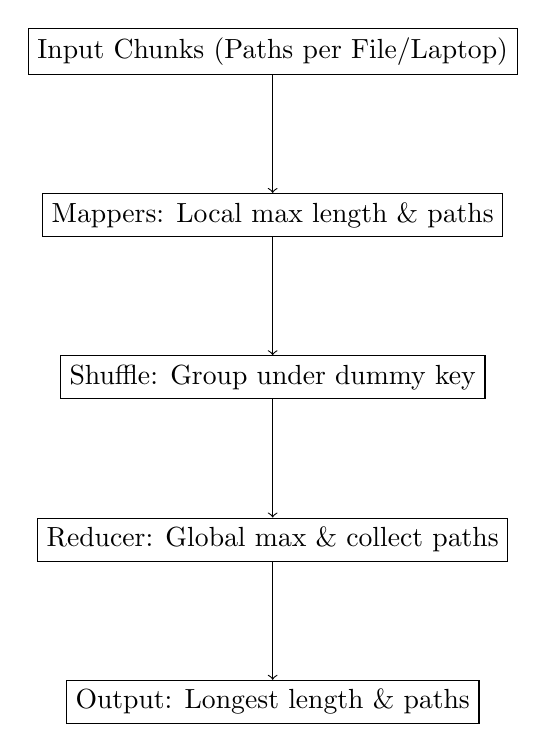
\begin{tikzpicture}
  \node[draw, rectangle] (input) {Input Chunks (Paths per File/Laptop)};
  \node[draw, rectangle, below=of input, yshift=-0.5cm] (map) {Mappers: Local max length \& paths};
  \node[draw, rectangle, below=of map, yshift=-0.5cm] (shuffle) {Shuffle: Group under dummy key};
  \node[draw, rectangle, below=of shuffle, yshift=-0.5cm] (reduce) {Reducer: Global max \& collect paths};
  \node[draw, rectangle, below=of reduce, yshift=-0.5cm] (output) {Output: Longest length \& paths};
  \draw[->] (input.south) -- (map.north);
  \draw[->] (map.south) -- (shuffle.north);
  \draw[->] (shuffle.south) -- (reduce.north);
  \draw[->] (reduce.south) -- (output.north);
\end{tikzpicture}
\caption{Mapper and Reducer Workflow}
\label{fig:workflow}
\end{figure}

\section{Who Does What}
\begin{itemize}
  \item \textbf{Mapper}: Analyzes a chunk of paths, determines the local maximum length, collects paths matching it, and emits them with a dummy key.
  \item \textbf{Shuffle/Sort}: Groups all mapper outputs under the single dummy key for reduction.
  \item \textbf{Reducer}: Compares local maxima to find the global maximum length, then gathers all paths from the locals that equal the global max.
  \item \textbf{Main Function}: Splits inputs into chunks (one per simulated file/laptop), coordinates map/shuffle/reduce, and outputs the result.
\end{itemize}

\end{document}